% report.tex

% !TEX program = pdflatex
% change it to xelatex if you use Chinese
\documentclass[]{beamer}

% preamble.tex

%%%%%%%%%%%%%%% Theme %%%%%%%%%%%%%%%
\usetheme{CambridgeUS} % try Madrid
\usecolortheme{beaver} % try beaver, dolphin, seahorse
% \usefonttheme[onlymath]{serif} % try "professionalfonts"
\usefonttheme{serif}  % standard font (same with that in ``standalone'')
% \setCJKmainfont{Microsoft YaHei} % try SimSun
% \setmainfont{Gill Sans}
% \setsansfont{Gill Sans}

\usepackage[export]{adjustbox}

\setbeamersize{text margin left = 2em, text margin right = 1em}
\setbeamercolor{footnote mark}{fg = teal}
\setbeamertemplate{itemize items}[default]
\setbeamertemplate{enumerate items}[default]

\renewcommand*{\thefootnote}{\alph{footnote}}
%%%%%%%%%%%%%%% Theme %%%%%%%%%%%%%%%

\usepackage{graphicx, subcaption}

\usepackage{amssymb, pifont}
\newcommand{\cmark}{\ding{51}}
\newcommand{\xmark}{\ding{55}}

%%%%%%%%%%%%%%% Algorithms %%%%%%%%%%%%%%%
\usepackage{algorithm}
\usepackage[noend]{algpseudocode}
% for two-column algorithms
% see https://tex.stackexchange.com/a/159431.
\usepackage{varwidth}

\newcommand{\code}[2]{#1:#2}
\newcommand{\hStatex}[0]{\vspace{4pt}}
\renewcommand\algorithmicthen{}
\renewcommand\algorithmicdo{}
%%%%%%%%%%%%%%% Algorithms %%%%%%%%%%%%%%%

%%%%%%%%%%%%%%% Theorems %%%%%%%%%%%%%%%
% theorems (global numbering)
\theoremstyle{definition}
\newtheorem{property}[theorem]{Property}
\newtheorem{assumption}{\textsc{Assumption}}
%%%%%%%%%%%%%%% Theorems %%%%%%%%%%%%%%%

\usepackage{caption}
\DeclareCaptionLabelSeparator{none}{}
\captionsetup{labelsep = none}

\makeatletter
\let\@@magyar@captionfix\relax
\makeatother

%%%%%%%%%%%%%%% Tables %%%%%%%%%%%%%%%
\usepackage{multirow}
\newcommand{\incell}[2]{\begin{tabular}[c]{@{}c@{}}#1\\[3pt] #2\end{tabular}}
%%%%%%%%%%%%%%% Tables %%%%%%%%%%%%%%%

%%%%%%%%%%%%%%% Figures %%%%%%%%%%%%%%%
% for fig without caption: #1: width/size; #2: fig file
\newcommand{\fig}[2]{
  \begin{figure}[htp]
    \centering
    \includegraphics[#1]{#2}
  \end{figure}
}

% for fig with caption: #1: width/size; #2: fig file; #3: fig caption
\newcommand{\figcap}[3]{
  \begin{figure}[htp]
    \centering
    \includegraphics[#1]{#2}
    \caption{#3}
  \end{figure}
}

\newcommand{\figdouble}[6]{
  \begin{figure}[h]
    \centering
    \begin{subfigure}[c]{#1\textwidth}
        \centering
        \includegraphics[width = #2\textwidth]{#3}
    \end{subfigure}
    \hfill
    \begin{subfigure}[c]{#4\textwidth}
        \centering
        \includegraphics[width = #5\textwidth]{#6}
    \end{subfigure}
  \end{figure}
}
%%%%%%%%%%%%%%% Figures %%%%%%%%%%%%%%%

%%%%%%%%%%%%%%% TiKZ %%%%%%%%%%%%%%%
\usepackage{tikz}
\usetikzlibrary{calc, trees, positioning, arrows, arrows.meta,
  chains, shapes.geometric, decorations.pathreplacing,
  decorations.pathmorphing, shapes, matrix, shapes.symbols, fit}
\tikzset{onslide/.code args={<#1>#2}{%
  \only<#1>{\pgfkeysalso{#2}} % \pgfkeysalso doesn't change the path
}}
\tikzset{temporal/.code args={<#1>#2#3#4}{%
  \temporal<#1>{\pgfkeysalso{#2}}{\pgfkeysalso{#3}}{\pgfkeysalso{#4}} % \pgfkeysalso doesn't change the path
}}

\usepackage[linewidth = 1pt, framemethod = TikZ]{mdframed}
\mdfsetup{frametitlealignment=\center}
%%%%%%%%%%%%%%% TiKZ %%%%%%%%%%%%%%%

%%%%%%%%%%%%%%% Citation %%%%%%%%%%%%%%%
% try "backend = bibtex", "backend = biber"
\usepackage[natbib = true, backend = biber, style = authoryear, maxbibnames = 99]{biblatex}
\setbeamertemplate{bibliography item}[article]
\renewcommand*{\bibfont}{\footnotesize}
\addbibresource{vldb2023-polysi-report.bib}

\newcommand{\ncite}[1]{\violet{\footnotesize [\cite{#1}]}}
%%%%%%%%%%%%%%% Citation %%%%%%%%%%%%%%%

%%%%%%%%%%%%%%% Colors %%%%%%%%%%%%%%%
\usepackage{xcolor}

\definecolor{DarkRed}{rgb}{0.55, 0.0, 0.0}

\newcommand{\red}[1]{\textcolor{red}{#1}}
\newcommand{\green}[1]{\textcolor{green}{#1}}
\newcommand{\blue}[1]{\textcolor{blue}{#1}}
\newcommand{\purple}[1]{\textcolor{purple}{#1}}
\newcommand{\cyan}[1]{\textcolor{cyan}{#1}}
\newcommand{\violet}[1]{\textcolor{violet}{#1}}
\newcommand{\lgray}[1]{\textcolor{lightgray}{#1}}
\newcommand{\teal}[1]{\textcolor{teal}{#1}}
\newcommand{\brown}[1]{\textcolor{brown}{#1}}
\newcommand{\orange}[1]{\textcolor{orange}{#1}}
\newcommand{\yellow}[1]{\textcolor{yellow}{#1}}

\newcommand{\hl}[2]{\fcolorbox{#1}{#1!60}{#2}}
%%%%%%%%%%%%%%% Colors %%%%%%%%%%%%%%%

%%%%%%%%%%%%%%% thankyou %%%%%%%%%%%%%%%
\newcommand{\thankyou}{
  \begin{frame}[noframenumbering]
    \begin{center}
      \fig{width = 0.618\textwidth}{figs/thankyou}
      \vspace{0.30cm}
      Hengfeng Wei (hfwei@nju.edu.cn)
    \end{center}
  \end{frame}
}
%%%%%%%%%%%%%%% thankyou %%%%%%%%%%%%%%%
% newcommands.tex

%%%%%%%%%%%%%%% Maths %%%%%%%%%%%%%%%
\newcommand{\N}{\mathbb{N}}
\newcommand{\Z}{\mathbb{Z}}
\newcommand{\set}[1]{\{#1\}}
\newcommand{\bset}[1]{\big\{#1\big\}}
\newcommand{\ps}{\mathcal{P}} % for powerset
\newcommand{\emptyseq}{\emptyset} % or using <>?
\newcommand{\tuple}[1]{\langle#1\rangle} % or using (#1)?
\newcommand{\btuple}[1]{\big\langle#1\big\rangle}
%%%%%%%%%%%%%%% Maths %%%%%%%%%%%%%%%

\usepackage{amssymb, latexsym}
\usepackage{bbding} % for checkmark and xsolid
\usepackage{mathtools}

\newcommand{\post}{\mathit{post}}
\newcommand{\comment}{\mathit{comment}}
\newcommand{\emptypost}{\mathit{empty}}
\newcommand{\acct}{\brown{\mathit{acct}}}
\newcommand{\acctone}{\brown{\mathit{acct}_{1}}}
\newcommand{\accttwo}{\brown{\mathit{acct}_{2}}}

\newcommand{\yes}{\green{\Checkmark}}
\newcommand{\no}{\red{\XSolidBrush}}

\newcommand{\Key}{{\sf Key}}
\newcommand{\Val}{{\sf Val}}

\newcommand{\h}{\mathcal{H}}
%%%%%%%%%%%%%%% system models %%%%%%%%%%%%%%%
\newcommand{\E}{E}
\newcommand{\evar}{\mathit{e}}
\newcommand{\fvar}{\mathit{f}}
\newcommand{\Event}{{\sf Event}}
\newcommand{\REvent}{{\sf REvent}}
\newcommand{\WEvent}{{\sf WEvent}}
\newcommand{\HEvent}{{\sf HEvent}}
\newcommand{\op}{{\sf op}}
\newcommand{\Op}{{\sf Op}}
\newcommand{\opvar}{\mathit{op}}
\newcommand{\readevent}{{\sf R}}
\newcommand{\Read}{{\sf Read}\;}
\newcommand{\writeevent}{{\sf W}}
\newcommand{\Write}{{\sf Write}\;}
\newcommand{\WriteTx}{{\sf WriteTx}}
\newcommand{\W}{{\sf W}}
\newcommand{\R}{{\sf R}}
\newcommand{\T}{T}
%%%%%%%%%%%%%%% system models %%%%%%%%%%%%%%%

%%%%%%%%%%%%%%% axioms %%%%%%%%%%%%%%%
\renewcommand{\ae}{\mathcal{A}}
\newcommand{\axiom}{\Phi}
\newcommand{\rel}[1]{\xrightarrow{#1}}
\newcommand{\comp}{\;;\;}
\newcommand{\po}{{\sf po}}
\newcommand{\so}{\textsc{so}}
\newcommand{\rb}{\textsc{rb}}
\newcommand{\cb}{\textsc{cb}}
\newcommand{\vis}{\textsc{vis}}
\newcommand{\ar}{\textsc{ar}}
\newcommand{\hist}{\text{Hist}}
\newcommand{\intaxiom}{\textsc{Int}}
\newcommand{\extaxiom}{\textsc{Ext}}
\newcommand{\sessionaxiom}{\textsc{Session}}
\newcommand{\prefixaxiom}{\textsc{Prefix}}
\newcommand{\conflict}{\bowtie}
\newcommand{\noconflictaxiom}{\textsc{NoConflict}}
%%%%%%%%%%%%%%% axioms %%%%%%%%%%%%%%%

%%%%%%%%%%%%%%% consistency models %%%%%%%%%%%%%%%
\newcommand{\si}{\textsc{SI}}
\newcommand{\ser}{\textsc{SER}}
%%%%%%%%%%%%%%% consistency models %%%%%%%%%%%%%%%

%%%%%%%%%%%%%%% pseudo-code %%%%%%%%%%%%%%%
\newcommand{\g}{G}
\newcommand{\inducedgraph}{I}
\newcommand{\eithervar}{\mathit{either}}
\newcommand{\orvar}{\mathit{or}}
\newcommand{\reachability}{\textsc{Reachability}}
\newcommand{\reachabilityvar}{\mathit{reachability}}

\newcommand{\vertex}{\mathsf{Vertex}}
\newcommand{\edges}{\mathsf{Edge}}
\newcommand{\cons}{\mathsf{Cons}}

\newcommand{\vvar}{\mathit{v}}
\newcommand{\precvar}{\mathit{prec}}
\newcommand{\egvar}{\mathit{e}}
\newcommand{\edgevar}{\mathit{edge}}
\newcommand{\cvar}{\mathit{c}}
\newcommand{\consvar}{\mathit{cons}}

\newcommand{\BV}{\mathsf{BV}}
\newcommand{\Clause}{\mathsf{Cl}}
\newcommand{\DV}{\mathsf{DV}}
\newcommand{\formula}{\mathcal{F}}

\newcommand{\fromvar}{\mathit{from}}
\newcommand{\tovar}{\mathit{to}}
\newcommand{\typevar}{\mathit{type}}

\newcommand{\graphA}{\mathit{Dep}}
\newcommand{\graphB}{\mathit{AntiDep}}
\newcommand{\knowninducedgraph}{\mathit{KI}}
%%%%%%%%%%%%%%% pseudo-code %%%%%%%%%%%%%%%

%%%%%%%%%%%%%%% proof %%%%%%%%%%%%%%%
\newcommand{\inv}{\textsc{Inv}\;}
\newcommand{\case}{\textsc{Case}}
\newcommand{\casei}{\case\; I}
\newcommand{\caseii}{\case\; II}
%%%%%%%%%%%%%%% proof %%%%%%%%%%%%%%%

%%%%%%%%%%%%%%% checking %%%%%%%%%%%%%%%
\providecommand{\G}{}
\renewcommand{\G}{\mathcal{G}}
\renewcommand{\H}{\mathcal{H}}

\newcommand{\SO}{\textup{\textsf{SO}}}
\newcommand{\WR}{\textup{\textsf{WR}}}
\newcommand{\WW}{\textup{\textsf{WW}}}
\newcommand{\RW}{\textup{\textsf{RW}}}
\newcommand{\GraphSI}{\textsf{GraphSI}}
\newcommand{\HistSI}{\textsf{HistSI}}
%%%%%%%%%%%%%%% checking %%%%%%%%%%%%%%%

\newcommand{\polysi}{\textsc{PolySI}}
\newcommand{\cobra}{\textsc{Cobra}}

\newcommand{\keyxvar}{\textcolor{cyan}{\mathit{x}}}
\newcommand{\keyyvar}{\textcolor{brown}{\mathit{y}}}
%%%%%%%%%%%%%%%%%%%%%%%%%%%%%%%%%%%%%%%%%%%%%%%%%%%%%%%%%%%%%%%%%%%%%%%%%%%%%%%%
\title[]{Efficient Black-box Checking of Snapshot Isolation in Databases}
\subtitle{\teal{(Conference VLDB'2024)}}

\author[Hengfeng Wei]{Hengfeng Wei}
\titlegraphic{
  
\includegraphics[height = 1.5cm]{figs/nju-logo-purple}~
  
\includegraphics[height = 1.5cm]{figs/software-logo}}
\institute{hfwei@nju.edu.cn}
\date{\today}
%%%%%%%%%%%%%%%%%%%%
\begin{document}
\maketitle
%%%%%%%%%%%%%%%%%%%%
% intro.tex

%%%%%%%%%%%%%%%%%%%%
\begin{frame}{Transaction and Isolation Level}
  \begin{center}
    A transaction is a \blue{\it group} of operations
    that are executed \red{atomically}.

    \vspace{0.30cm}
		\resizebox{0.55\textwidth}{!}{% isolation-intro-write-skew-tikz.tex

\begin{tikzpicture}[
  node distance = 1.5cm and 1.5cm,
  txn/.style = {draw, inner sep = 3pt, align = left},
  comm/.style = {arrows = {Stealth-Stealth}, ultra thick, purple}]

  \uncover<2->{
  \node[txn] (t-alice)
    {$x_{1} \gets \readevent(\acctone)$\\[2pt]
     $x_{2} \gets \readevent(\accttwo)$\\[2pt]
     $\text{\bf if}\; x_{1} + x_{2} > 100$ \\[2pt]
     $\quad \red{x_{1} \gets x_{1} - 100}$ \\[2pt]
     $\quad \writeevent(\acctone, x_{1})$};
  }

  \node[txn, right = of t-alice] (t-bob)
    {$x_{1} \gets \readevent(\acctone)$\\[2pt]
     $x_{2} \gets \readevent(\accttwo)$\\[2pt]
     $\text{\bf if}\; x_{1} + x_{2} > 100$ \\[2pt]
     $\quad \red{x_{2} \gets x_{2} - 100}$ \\[2pt]
     $\quad \writeevent(\accttwo, x_{2})$};

  \uncover<2->{
  \node[txn, right = of t-bob] (t-carol)
    {$x_{1} \gets \readevent(\acctone)$\\[2pt]
     $x_{2} \gets \readevent(\accttwo)$};
  }

  \uncover<3->{
  \node[draw, fill = yellow!50, below = of t-bob, font = \large,
    inner sep = 8pt] (isolation)
    {{Isolation Level (aka Transactional Consistency Model)}};
  }

  \node[below = of isolation,
    label = {[label distance = 5pt]above : {\large $\acctone = \accttwo = 60$}}] (db)
    {
\includegraphics[scale = 0.75]{figs/db-logo-dollar}};

  \uncover<1>{
  \draw[comm] (t-bob) -- (db);
  }

  \uncover<3->{
  \draw[comm] (t-alice) -- (t-alice |- isolation.north);
  \draw[comm] (t-bob) -- (t-bob |- isolation.north);
  \draw[comm] (t-carol) -- (t-carol |- isolation.north);
  \draw[comm] (isolation) -- (isolation |- db.north);
  }
\end{tikzpicture}}

    \vspace{0.20cm}
    The isolation levels specify how concurrent transactions \\[2pt]
    are isolated from each other.
  \end{center}
\end{frame}
%%%%%%%%%%%%%%%%%%%%

%%%%%%%%%%%%%%%%%%%%
\begin{frame}{Serializability (SER)}
  \begin{center}
    All transactions appear to be executed in some total order.

    \vspace{0.30cm}
		\resizebox{0.50\textwidth}{!}{% isolation-ser-write-skew-tikz.tex

\begin{tikzpicture}[
  node distance = 1.5cm and 1.5cm,
  txn/.style = {draw, inner sep = 3pt, align = center},
  comm/.style = {arrows = {Stealth-Stealth}, ultra thick, purple}]

  \node[txn] (t-alice)
    {$x_{1} \gets \readevent(\acctone)$\\[2pt]
     $x_{2} \gets \readevent(\accttwo)$\\[2pt]
     $\text{\bf if}\; x_{1} + x_{2} > 100$ \\[2pt]
     $\quad \red{x_{1} \gets x_{1} - 100}$ \\[2pt]
     $\quad \writeevent(\acctone, x_{1})$};

  \node[txn, right = of t-alice] (t-bob)
    {$x_{1} \gets \readevent(\acctone)$\\[2pt]
     $x_{2} \gets \readevent(\accttwo)$\\[2pt]
     $\text{\bf if}\; x_{1} + x_{2} > 100$ \\[2pt]
     $\quad \red{x_{2} \gets x_{2} - 100}$ \\[2pt]
     $\quad \writeevent(\accttwo, x_{2})$};

  \node[txn, right = of t-bob] (t-carol)
    {$x_{1} \gets \readevent(\acctone)$\\[2pt]
     $x_{2} \gets \readevent(\accttwo)$};

  \node[draw, fill = yellow!50, below = of t-bob, font = \large,
    inner sep = 8pt, minimum width = 260pt] (isolation)
    {{Serializability (SER)}};

  \node[below = of isolation,
    label = {[label distance = 5pt]above : {\large $\acctone = \accttwo = 60$}}] (db)
    {
\includegraphics[scale = 0.70]{figs/db-logo-dollar}};

  \draw[comm] (t-alice) -- (t-alice |- isolation.north);
  \draw[comm] (t-bob) -- (t-bob |- isolation.north);
  \draw[comm] (t-carol) -- (t-carol |- isolation.north);
  \draw[comm] (isolation) -- (isolation |- db.north);

  \uncover<3->{
  \node[txn, below = 0.50cm of db, fill = green!30] (t-bob-execution)
    {$\readevent(\acctone, 60)$ \\[2pt]
     $\readevent(\accttwo, 60)$};
  }

  \uncover<2->{
  \node[txn, left = of t-bob-execution] (t-alice-execution)
    {$\readevent(\acctone, 60)$ \\[2pt]
     $\readevent(\accttwo, 60)$ \\[2pt]
     $\writeevent(\acctone, -40)$};
  }

  \uncover<4->{
  \node[txn, right = of t-bob-execution] (t-carol-execution)
    {$\readevent(\acctone, 60)$ \\[2pt]
     $\readevent(\accttwo, 60)$};
  }
\end{tikzpicture}}

    \vspace{0.20cm}
    However, implementing serializability is too expensive.
  \end{center}
\end{frame}
%%%%%%%%%%%%%%%%%%%%

%%%%%%%%%%%%%%%%%%%%
\begin{frame}{Snapshot Isolation (SI)}
  \begin{center}
		\resizebox{0.50\textwidth}{!}{% isolation-si-write-skew-tikz.tex

\begin{tikzpicture}[
  node distance = 1.5cm and 1.5cm,
  txn/.style = {draw, inner sep = 3pt, align = center},
  comm/.style = {arrows = {Stealth-Stealth}, ultra thick, purple}]

  \node[txn] (t-alice)
    {$x_{1} \gets \readevent(\acctone)$\\[2pt]
     $x_{2} \gets \readevent(\accttwo)$\\[2pt]
     $\text{\bf if}\; x_{1} + x_{2} > 100$ \\[2pt]
     $\quad \red{x_{1} \gets x_{1} - 100}$ \\[2pt]
     $\quad \writeevent(\acctone, x_{1})$};

  \node[txn, right = of t-alice] (t-bob)
    {$x_{1} \gets \readevent(\acctone)$\\[2pt]
     $x_{2} \gets \readevent(\accttwo)$\\[2pt]
     $\text{\bf if}\; x_{1} + x_{2} > 100$ \\[2pt]
     $\quad \red{x_{2} \gets x_{2} - 100}$ \\[2pt]
     $\quad \writeevent(\accttwo, x_{2})$};

  \node[txn, right = of t-bob] (t-carol)
    {$x_{1} \gets \readevent(\acctone)$\\[2pt]
     $x_{2} \gets \readevent(\accttwo)$};

  \node[draw, fill = yellow!50, below = of t-bob, font = \large,
    inner sep = 8pt, minimum width = 260pt] (isolation)
    {{Snapshot Isolation (SI)}};

  \node[below = of isolation,
    label = {[label distance = 5pt]above : {\large $\acctone = \accttwo = 60$}}] (db)
    {
\includegraphics[scale = 0.70]{figs/db-logo-dollar}};

  \draw[comm] (t-alice) -- (t-alice |- isolation.north);
  \draw[comm] (t-bob) -- (t-bob |- isolation.north);
  \draw[comm] (t-carol) -- (t-carol |- isolation.north);
  \draw[comm] (isolation) -- (isolation |- db.north);

  \uncover<2->{
  \node[txn, below = 0.50cm of db, fill = green!30] (t-bob-execution)
    {$\readevent(\acctone, 60)$ \\[2pt]
     $\readevent(\accttwo, 60)$ \\[2pt]
     $\writeevent(\accttwo, -40)$};
  }
  \uncover<2->{
  \node[txn, left = of t-bob-execution] (t-alice-execution)
    {$\readevent(\acctone, 60)$ \\[2pt]
     $\readevent(\accttwo, 60)$ \\[2pt]
     $\writeevent(\acctone, -40)$};
  }
  \uncover<3->{
  \node[txn, right = of t-bob-execution, fill = red!30] (t-carol-execution)
    {$\readevent(\acctone, -40)$ \\[2pt]
     $\readevent(\accttwo, -40)$};

    \node[above = 1.50cm of t-carol-execution] (write-skew)
      {\green{\Large \textsc{Write Skew}}};
    \node[above = 0.80cm of t-carol-execution, scale = 3] (yes) {\yes};
  }
\end{tikzpicture}}

    \vspace{0.20cm}
    \violet{Snapshot Read:} Each transaction reads data from a {\it snapshot} \\
      as of the time the transaction started.
  \end{center}
\end{frame}
%%%%%%%%%%%%%%%%%%%%

%%%%%%%%%%%%%%%%%%%%
\begin{frame}{Snapshot Isolation (SI)}
  \begin{center}
    \resizebox{0.48\textwidth}{!}{% isolation-si-lost-update-tikz.tex

\begin{tikzpicture}[
  node distance = 1.5cm and 1.5cm,
  txn/.style = {draw, inner sep = 3pt, align = center},
  comm/.style = {arrows = {Stealth-Stealth}, ultra thick, purple}]

  \node[txn] (t-alice)
    {$x \gets \readevent(\acct)$ \\[2pt]
     $x \gets x + 50$ \\[2pt]
     $\writeevent(\acct, x)$};

  \node[txn, right = of t-alice] (t-bob)
    {$x \gets \readevent(\acct)$ \\[2pt]
     $x \gets x + 25$ \\[2pt]
     $\writeevent(\acct, x)$};

  \node[txn, right = of t-bob] (t-carol)
    {$\readevent(\acct)$};

  \node[draw, fill = yellow!50, below = of t-bob, font = \large,
    inner sep = 8pt, minimum width = 260pt] (isolation)
    {{Snapshot Isolation (SI)}};

  \node[below = of isolation,
    label = {[label distance = 5pt]above : {\large $\acct = 0$}}] (db)
    {
\includegraphics[scale = 0.70]{figs/db-logo-dollar}};

  \draw[comm] (t-alice) -- (t-alice |- isolation.north);
  \draw[comm] (t-bob) -- (t-bob |- isolation.north);
  \draw[comm] (t-carol) -- (t-carol |- isolation.north);
  \draw[comm] (isolation) -- (isolation |- db.north);

  \uncover<2->{
  \node[txn, below = 0.50cm of db] (t-bob-execution)
    {$\readevent(\acct, 0)$ \\[2pt] $\writeevent(\acct, ?)$};
  \node[below = 0.50cm of db, scale = 3.00] (t-bob-abort) {\no};
  }
  % \uncover<6->{
  % \node[txn, below = 0.50cm of db, fill = green!50] (t-bob-retry)
  %   {$\readevent(\acct, 0)$ \\[2pt] $\writeevent(\acct, 75)$};
  % }

  \uncover<2->{
  \node[txn, left = of t-bob-execution] (t-alice-execution)
    {$\readevent(\acct, 0)$ \\[2pt] $\writeevent(\acct, 50)$};
  }

  \uncover<2->{
  \node[above right = 0.20cm and 1.00cm of t-bob-execution] (lost-update)
    {\red{\large \textsc{Lost Update}}};
  \node[above right = -0.60cm and 1.30cm of t-bob-execution, scale = 3] (no) {\no};
  }
\end{tikzpicture}}
  \end{center}

  \vspace{-0.50cm}
  \violet{Snapshot Write:}
    Concurrent transactions {\it cannot} write to the same key.
    One of them must be aborted.
\end{frame}
%%%%%%%%%%%%%%%%%%%%

%%%%%%%%%%%%%%%%%%%%
% \begin{frame}{Snapshot Isolation (SI)}
%   \begin{center}
%     \resizebox{0.60\textwidth}{!}{% isolation-si-causality-violation-tikz.tex

\begin{tikzpicture}[
  node distance = 1.5cm and 1.5cm,
  txn/.style = {draw, inner sep = 3pt, align = center},
  comm/.style = {arrows = {Stealth-Stealth}, ultra thick, purple}]

  \node[] (t-bob) {
\includegraphics[scale = 0.08]{figs/social-network-logo}};

  \node[draw, fill = yellow!50, below = of t-bob, font = \large,
    inner sep = 8pt, minimum width = 260pt] (isolation)
    {{Snapshot Isolation (SI)}};

  \node[below = of isolation] (db)
    {
\includegraphics[scale = 0.70]{figs/db-logo-dollar}};

  \draw[comm] (t-bob) -- (t-bob |- isolation.north);
  \draw[comm] (isolation) -- (isolation |- db.north);

  \uncover<3->{
  \node[txn, below = 0.50cm of db] (t-bob-execution)
    {$\readevent(\keyxvar, \post)$ \\[2pt] $\writeevent(\keyyvar, \comment)$};
  }

  \uncover<2->{
  \node[txn, left = of t-bob-execution] (t-alice-execution)
    {$\writeevent(\keyxvar, \post)$};
  }

  \uncover<4->{
  \node[txn, right = of t-bob-execution, fill = red!30] (t-carol-execution)
    {$\readevent(\keyxvar, \emptypost)$ \\[2pt] $\readevent(\keyyvar, \comment)$};
  }
  \uncover<6->{
  \node[right = 0.10cm of t-carol-execution, scale = 2] (no-carol) {\no};
  }

  \uncover<5->{
  \node[above = of t-carol-execution] (causality-violation)
    {\red{\large \textsc{Causality Violation}}};
  }
  \uncover<6->{
  \node[above = 0.60cm of t-carol-execution, scale = 3] (no) {\no};
  }
\end{tikzpicture}}
%   \end{center}
% \end{frame}
%%%%%%%%%%%%%%%%%%%%

%%%%%%%%%%%%%%%%%%%%
\begin{frame}{Database Systems and Snapshot Isolation}
  \begin{center}
    Many database systems implement snapshot isolation.

    \vspace{0.30cm}
    \fig{width = 0.80\textwidth}{figs/db-si}
  \end{center}
\end{frame}
%%%%%%%%%%%%%%%%%%%%

%%%%%%%%%%%%%%%%%%%%
\begin{frame}{Database Systems and Snapshot Isolation}
  \begin{center}
    Database systems may \red{fail} to provide snapshot isolation correctly.

    \vspace{0.30cm}
    \fig{width = 0.85\textwidth}{figs/db-si-violations}
  \end{center}
\end{frame}
%%%%%%%%%%%%%%%%%%%%

%%%%%%%%%%%%%%%%%%%%
\begin{frame}{The SI Checking Problem}
  \begin{definition}[The SI Checking Problem]
    The SI checking problem is the \purple{decision problem} of determing \\[5pt]
    whether a \teal{{\it history} $\H = (T, \SO)$}\footnote{
      We take the common ``UniqueValue'' assumption on histories:
      for each key, every write to the key assigns a unique value.
    } of a database system satisfies SI?
  \end{definition}

  \fig{width = 0.60\textwidth}{figs/si-checking}

  \vspace{-0.50cm}
  \[
    \SO: \text{{\it session order} among the set $T$ of transactions}
  \]
\end{frame}
%%%%%%%%%%%%%%%%%%%%

%%%%%%%%%%%%%%%%%%%%
\begin{frame}{The SI Checking Problem}
  \begin{center}
    \uncover<1->{
      \blue{\it Sound:} If the checker says \no,
        then the history does {\it not} satisfy SI.
    }

    \vspace{0.20cm}
    \uncover<2->{
      \blue{\it Complete:} If the checker says \yes,
        then the history {\it satisfies} SI.
    }

    \vspace{0.30cm}
    % checker-tikz.tex

\begin{tikzpicture}[
  node distance = 0.5cm and 1.0cm,
  every label/.style = {font = \normalsize}]

	\node[draw, thick, inner sep = 8pt] (checker) {SI Checker};

	\coordinate (anchor) at ($(checker.west) + (-2.5, 0)$);
	\draw[->, thick] (anchor) to
	  node[above]{A history}
	  node[below]{$\H = (\T, \SO)$}
		(checker);

	\node[above right = of checker] (sat) {\yes};
	\node[below right = of checker] (unsat) {\no};

	\draw[->, thick] (checker) to (sat);
	\draw[->, thick] (checker) to (unsat);

	\uncover<1->{
		\node[above = 0.30cm of checker, blue] (sound) {\it Sound};
	}
	\uncover<2->{
		\node[below = 0.30cm of checker, blue] (complete) {\it Complete};
	}
	\uncover<3->{
		\node[right = 0.30cm of checker, blue] (efficient) {\it Efficient};
	}
	\uncover<4->{
		\node[below = 0.00cm of unsat, blue] (informative) {\it Informative};
	}
\end{tikzpicture}
    \vspace{0.30cm}

    \uncover<3->{
      \blue{\it Efficient:} The checker should {\it scale} up to large workloads.
    }

    \vspace{0.20cm}
    \uncover<4>{
      \blue{\it Informative:} The checker should provide
        understandable {\it counterexamples} if it finds violations.
    }
  \end{center}
\end{frame}
%%%%%%%%%%%%%%%%%%%%

%%%%%%%%%%%%%%%%%%%%
\begin{frame}{Related Work}
  \begin{description}
    \setlength{\itemsep}{15pt}
    \item[dbcop~\ncite{Complexity:OOPSLA2019}] checker for SI \\[2pt]
      not practically efficient; \\[2pt]
      not informative, returning only ``\textsf{False}'' upon violations
    \item[Cobra~\ncite{Cobra:OSDI2020}] state-of-the-art checker for SER \\[2pt]
      The SI checking problem is {\it harder}.
  \end{description}
\end{frame}
%%%%%%%%%%%%%%%%%%%%

%%%%%%%%%%%%%%%%%%%%
\begin{frame}{Related Work}
  \begin{description}
    \item[Elle~\ncite{Elle:VLDB2020}] checker for various isolation levels \\[2pt]

      \vspace{0.20cm}
      Work perfectly on traceable and recoverable histories;
      but may be incomplete on the key-value datatype

      \pause
      \vspace{0.20cm}
      SI checking based on the Adya-style notions~\ncite{Adya:PhDThesis1999}
      relies on the start/commit timestamps of transactions.\\[2pt]

      \pause
      \vspace{0.20cm}
      SI checking based on the~\ncite{AnalysingSI:JACM2018} notions
      may miss SI violations.\footnote{
        Could Elle tell the difference between snapshot isolation and strong-session-snapshot-isolation? https://github.com/jepsen-io/elle/issues/17}
        \footnote{Elle may miss two types of transaction anomalies. https://github.com/jepsen-io/elle/issues/21}
  \end{description}
\end{frame}
%%%%%%%%%%%%%%%%%%%%

%%%%%%%%%%%%%%%%%%%%
\begin{frame}{Contribution: the \polysi{} Checker}
  \fig{width = 0.70\textwidth}{figs/checker-polysi}
\end{frame}
%%%%%%%%%%%%%%%%%%%%

%%%%%%%%%%%%%%%%%%%%
\begin{frame}{Contribution: the \polysi{} Checker}
  \begin{center}
    % polysi-checker-tikz.tex

\begin{tikzpicture}[
  node distance = 0.5cm and 1.0cm,
  every label/.style = {font = \normalsize}]

	\node[draw, thick, inner sep = 8pt, fill = yellow!50] (polysi) {\textsc{PolySI}};

	\coordinate (anchor) at ($(polysi.west) + (-2.5, 0)$);
	\draw[->, thick] (anchor) to
	  node[above]{A history}
	  node[below]{$\H = (\T, \SO)$}
		(polysi);

	\node[above right = of polysi] (sat) {\yes};
	\node[below right = of polysi] (unsat) {\no};

	\draw[->, thick] (polysi) to (sat);
	\draw[->, thick] (polysi) to (unsat);

	\uncover<2->{
		\node[draw, below right = 1.50cm and 0.30cm of polysi.south, fill = brown!50, inner sep = 5pt, align = center]
			(monosat) {MonoSAT \\ Solving};
	}
	\uncover<1->{
		\node[draw, below left = 1.50cm and 0.30cm of polysi.south, fill = brown!50, inner sep = 5pt, align = center]
			(encoding) {SAT \\ Encoding};
	}
	\uncover<3->{
		\node[draw, left = 0.60cm of encoding, fill = brown!50, inner sep = 5pt, align = center]
			(pruning) {Constraints \\ Pruning};
	}
	\uncover<4->{
		\node[draw, right = 0.60cm of monosat, fill = brown!50, inner sep = 5pt, align = center]
			(counterexamples) {Counterexamples \\ Extracting};
	}
	\uncover<3->{
		\draw[->, thick, brown] (pruning) to (encoding);
	}
	\uncover<2->{
		\draw[->, thick, brown] (encoding) to (monosat);
	}
	\uncover<4->{
		\draw[->, thick, brown] (monosat) to (unsat);
		\draw[->, thick, brown] (unsat) to (counterexamples);
	}

	\uncover<1->{
		\draw[dashed, very thick, blue] (polysi.south west) to (pruning.north west);
		\draw[dashed, very thick, blue] (polysi.south east) to (counterexamples.north east);
	}
\end{tikzpicture}

    \vspace{0.50cm}
    \only<1>{
      \blue{{\it Sound} \&{\it Complete:}}
        a novel {\it polygraph} based characterization of SI
    }
    \only<2>{
      \blue{\it Efficient:} utilizing MonoSAT solver optimized for graph problems
    }
    \only<3>{
      \blue{\it Efficient:} pruning the constraints on {\it polygraph} before encoding
    }
    \only<4>{
      \blue{\it Informative:} extract counterexamples from the UNSAT core
    }
  \end{center}
\end{frame}
%%%%%%%%%%%%%%%%%%%%
% si.tex
% si-polygraph.tex

%%%%%%%%%%%%%%%%%%%%
\begin{frame}{Dependency Graph-based Characterization of SI}
  \begin{center}
		\only<4>{
			\red{\it Suppose that $T_{A} \rel{\WW} T_{B}$}
		}
		\only<5>{
			$T_{0} \rel{\WR} T_{A} \land T_{0} \rel{\WW} T_{B}
			  \implies T_{A} \rel{\RW} T_{B}$
		}
		\only<6>{
			$T_{0} \rel{\WR} T_{B} \land T_{0} \rel{\WW} T_{A}
			  \implies T_{A} \rel{\RW} T_{A}$
		}
		\only<7->{
			\red{$\boxed{\text{\it Suppose that}\;\; T_{A} \rel{\WW} T_{B}}$}
		}

		\vspace{0.20cm}
		{% banking-lost-update-dep-tikz.tex

\begin{tikzpicture}[
  node distance = 0.8cm and 2.0cm,
  wr/.style = {->, thick},
  ww/.style = {->, thick, dashed, red},
  rw/.style = {->, thick, dotted, blue},
  txn/.style = {draw, inner sep = 3pt, align = center}]

  \node[txn, label = above : $T_{0}$] (t) {$\writeevent(\acct, 0)$};

  \node[txn, label = above : $T_{A}$, above right = of t] (t-alice)
    {$\readevent(\acct, 0)$ \\[2pt] $\writeevent(\acct, 50)$};
  \node[txn, label = below : $T_{B}$, below right = of t] (t-bob)
    {$\readevent(\acct, 0)$ \\[2pt] $\writeevent(\acct, 25)$};

  \node[txn, label = above : $T'_{A}$, right = 6.0cm of t] (t-alice-read) {$\readevent(\acct, 25)$};

  \uncover<2->{
    \draw[wr, sloped] (t) to node[below]{$\WR$} (t-alice.west);
    \draw[wr, sloped] (t) to node[above]{$\WR$} (t-bob.west);
    \draw[wr, sloped] (t-bob.east) to node[below]{$\WR$} (t-alice-read.south);
  }

  \uncover<3->{
    \draw[ww, bend left, sloped] (t) to node[above]{$\WW$} (t-alice);
    \draw[ww, bend right, sloped] (t) to node[below]{$\WW$} (t-bob);
  }
  \uncover<4->{
    \draw[ww] (t-alice) to node[]{$\WW$} (t-bob);
  }

  \uncover<5->{
    \draw[rw, bend right = 60] (t-alice.-145) to node[]{$\RW$} (t-alice.-145 |- t-bob.north);
  }
  \uncover<6->{
    \draw[rw, bend right = 60] (t-bob.35) to node[]{$\RW$} (t-bob.35 |- t-alice.south);
  }
\end{tikzpicture}}
		\vspace{0.20cm}

		\only<2>{
			$\WR$: ``write-read'' dependency capturing the ``read-from'' relation
		}
		\only<3-4>{
			$\WW$: ``write-write'' dependency capturing the version order
		}
		\only<5-6>{
			$\RW$: ``read-write'' dependency capturing the overwritten relation
		}
		\only<7>{
			undesired cycle: $T_{A} \rel{\WW} T_{B} \rel{\RW} T_{A}$
		}
  \end{center}
\end{frame}
%%%%%%%%%%%%%%%%%%%%

%%%%%%%%%%%%%%%%%%%%
\begin{frame}{Dependency Graph-based Characterization of SI}
	\begin{center}
		\uncover<2->{
			\red{$\boxed{\text{\it Suppose that}\;\; T_{B} \rel{\WW} T_{A}}$}
		}

		\vspace{0.20cm}
		{% banking-lost-update-depgraph-ww-tbta-tikz.tex

\begin{tikzpicture}[
  node distance = 0.8cm and 2.0cm,
  wr/.style = {->, thick},
  ww/.style = {->, thick, dashed, red},
  rw/.style = {->, thick, dotted, blue},
  txn/.style = {draw, inner sep = 3pt, align = center}]

  \node[txn, label = above : $T_{0}$] (t) {$\writeevent(\acct, 0)$};

  \node[txn, label = above : $T_{A}$, above right = of t] (t-alice)
    {$\readevent(\acct, 0)$ \\[2pt] $\writeevent(\acct, 50)$};
  \node[txn, label = below : $T_{B}$, below right = of t] (t-bob)
    {$\readevent(\acct, 0)$ \\[2pt] $\writeevent(\acct, 25)$};

  \node[txn, label = above : $T'_{A}$, right = 6.0cm of t] (t-alice-read) {$\readevent(\acct, 25)$};

  \draw[wr, sloped] (t) to node[below]{$\WR$} (t-alice.west);
  \draw[wr, sloped] (t) to node[above]{$\WR$} (t-bob.west);
  \draw[wr, sloped] (t-bob.east) to node[below]{$\WR$} (t-alice-read.south);

  \draw[ww, bend left, sloped] (t) to node[above]{$\WW$} (t-alice);
  \draw[ww, bend right, sloped] (t) to node[below]{$\WW$} (t-bob);
  \uncover<2->{
  \draw[ww] (t-bob) to node[]{$\WW$} (t-alice);
  }

  \draw[rw, bend right = 60] (t-alice.-145) to node[]{$\RW$} (t-alice.-145 |- t-bob.north);
  \draw[rw, bend right = 60] (t-bob.35) to node[]{$\RW$} (t-bob.35 |- t-alice.south);

  \uncover<3->{
  \draw[rw] (t-alice-read.north) to node[sloped, above]{$\RW$} (t-alice.east);
  }
\end{tikzpicture}}
		\vspace{0.20cm}

		\uncover<5>{
			undesired cycle: $T_{B} \rel{\WW} T_{A} \rel{\RW} T_{B}$
		}
	\end{center}
\end{frame}
%%%%%%%%%%%%%%%%%%%%

%%%%%%%%%%%%%%%%%%%%
\begin{frame}{Dependency Graph-based Characterization of SI}
  \begin{center}
		We have considered both bases $T_{A} \rel{\WW} T_{B}$
		and $T_{B} \rel{\WW} T_{A}$.

		\vspace{0.20cm}
		\fig{width = 0.65\textwidth}{figs/banking-lost-update-wr}
		\vspace{0.20cm}

		Either case leads to an undesired cycle. \\[2pt]
		Therefore, it does not satisfy SI.
  \end{center}
\end{frame}
%%%%%%%%%%%%%%%%%%%%

%%%%%%%%%%%%%%%%%%%%
\begin{frame}{Dependency Graph-based Characterization of SI}
  \begin{theorem}[Theorem 4.1 of~\ncite{AnalysingSI:JACM2018}]
		Informally, a history satisfies SI if only if \\[3pt]
		\red{there exists} a dependency graph for it that contains \\[3pt]
		only cycles (if any) with \blue{at least two adjacent $\RW$} edges.
	\end{theorem}
\end{frame}
%%%%%%%%%%%%%%%%%%%%

%%%%%%%%%%%%%%%%%%%%
\begin{frame}{Dependency Graph-based Characterization of SI}
	\begin{columns}
		\column{0.50\textwidth}
			{\fig{width = 1.00\textwidth}{figs/banking-lost-update-depgraph}}
		\column{0.50\textwidth}
			{\fig{width = 1.00\textwidth}{figs/banking-lost-update-depgraph}}
	\end{columns}

	\vspace{0.30cm}
	\begin{center}
		Every possible dependency graph contains
		an undesired \raisebox{-1.0ex}{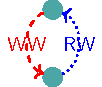
\includegraphics[scale = 0.50]{figs/ww-rw-cycle}} cycle.
	\end{center}
\end{frame}
%%%%%%%%%%%%%%%%%%%%

%%%%%%%%%%%%%%%%%%%%
\begin{frame}{Dependency Graph-based Characterization of SI}
  \begin{theorem}[Theorem 4.1 of~\ncite{AnalysingSI:JACM2018}]
		For a history \emph{$\H = (\T, \SO)$},
		\vspace{-0.30cm}
		\begin{align*}
			\H \models \si & \iff \H \models \intaxiom \;\land \\
				&\red{\exists}\; \WR, \WW, \RW.\; \G = (\H, \WR, \WW, \RW) \;\land \\
				&\quad (\blue{((\SO_{\G} \cup \WR_{\G} \cup \WW_{\G}) \comp \RW_{\G}?)} \text{\it\; is acyclic}).
		\end{align*}
  \end{theorem}

	\begin{center}
		\resizebox{0.60\textwidth}{!}{% banking-lost-update-dep-theorem-tikz.tex

\begin{tikzpicture}[
  node distance = 0.8cm and 2.0cm,
  wr/.style = {->, thick},
  ww/.style = {->, thick, dashed, red},
  rw/.style = {->, thick, dotted, blue},
  txn/.style = {draw, inner sep = 3pt, align = center},
  comp/.style = {->, ultra thick, purple, loosely dash dot}]

  \node[txn, label = above : $T_{0}$] (t) {$\writeevent(\acct, 0)$};

  \node[txn, label = above : $T_{A}$, above right = of t] (t-alice)
    {$\readevent(\acct, 0)$ \\[2pt] $\writeevent(\acct, 50)$};
  \node[txn, label = below : $T_{B}$, below right = of t] (t-bob)
    {$\readevent(\acct, 0)$ \\[2pt] $\writeevent(\acct, 25)$};

  \node[txn, label = above : $T'_{A}$, right = 6.0cm of t] (t-alice-read) {$\readevent(\acct, 25)$};

  \draw[wr, sloped] (t) to node[below]{$\WR$} (t-alice.west);
  \draw[wr, sloped] (t) to node[above]{$\WR$} (t-bob.west);
  \draw[wr, sloped] (t-bob.east) to node[below]{$\WR$} (t-alice-read.south);

  \draw[ww, bend left, sloped] (t) to node[above]{$\WW$} (t-alice);
  \draw[ww, bend right, sloped] (t) to node[below]{$\WW$} (t-bob);
  \draw[ww] (t-alice) to node[]{$\WW$} (t-bob);

  \uncover<1-2>{
  \draw[rw, bend right = 60] (t-alice.-145) to node[]{$\RW$} (t-alice.-145 |- t-bob.north);
  \draw[rw, bend right = 60] (t-bob.35) to node[]{$\RW$} (t-bob.35 |- t-alice.south);
  }

  \uncover<2->{
  \draw[comp, bend left = 30] (t.north west) to (t-alice.north west);
  }
  \uncover<2->{
  \draw[comp, bend right = 30] (t.south west) to (t-bob.south west);
  }
  \uncover<2->{
  \draw[comp] (t-alice.south east) to [out = -30, in = 30, looseness = 4] (t-alice.north east);
  }
\end{tikzpicture}}
	\end{center}
\end{frame}
%%%%%%%%%%%%%%%%%%%%

%%%%%%%%%%%%%%%%%%%%
\begin{frame}{Dependency Graph-based Characterization of SI}
  \begin{center}
		\red{$\mathcal{Q}:$ How to capture and resolve all {possible} $\WW$ dependencies?}

		\vspace{0.50cm}
		\begin{columns}
			\column{0.50\textwidth}
				\fig{width = 1.00\textwidth}{figs/banking-lost-update-depgraph}
			\column{0.50\textwidth}
				\fig{width = 1.00\textwidth}{figs/banking-lost-update-depgraph-ww-tbta}
		\end{columns}

		\pause
		\vspace{0.80cm}
		\blue{$\mathcal{A}:$ encode them into SAT formulas based on \\[2pt]
		  (generalized) polygraphs and solve them using SAT solvers.}
  \end{center}
\end{frame}
%%%%%%%%%%%%%%%%%%%%

%%%%%%%%%%%%%%%%%%%%
\begin{frame}{Polygraphs: A Family of Dependency Graphs}
	\begin{center}
		Consider the two cases of $\WW$ dependencies between $T_{A}$ and $T_{B}$.
	\end{center}

	\begin{columns}[c]
		\column{0.50\textwidth}
			\fig{width = 0.80\textwidth}{figs/banking-lost-update-depgraph}
		\column{0.50\textwidth}
			\fig{width = 0.80\textwidth}{figs/banking-lost-update-depgraph-ww-tbta}
	\end{columns}

	\begin{center}
		\pause
		\fig{width = 0.40\textwidth}{figs/banking-lost-update-polygraph}
		generalized polygraph:

		\pause
		\vspace{-0.30cm}
		\[
			\tuple{\teal{\eithervar} \triangleq \set{T_{A} \rel{\WW} T_{B}},
				\teal{\orvar} \triangleq \set{T_{B} \rel{\WW} T_{A}, T_{A}' \rel{\RW} T_{A}}}
		\]
	\end{center}
\end{frame}
%%%%%%%%%%%%%%%%%%%%

%%%%%%%%%%%%%%%%%%%%
\begin{frame}{\polysi: Pruning before Encoding (the $\WW$ case)}
	\begin{columns}
		\column{0.40\textwidth}
			\fig{width = 0.70\textwidth}{figs/pruning-ww-case}
		\column{0.60\textwidth}
		  \resizebox{1.00\textwidth}{!}{% banking-lost-update-polygraph-pruning-ww-tikz.tex

\begin{tikzpicture}[
  node distance = 0.8cm and 2.0cm,
  wr/.style = {->, thick},
  ww/.style = {->, thick, dashed, red},
  rw/.style = {->, thick, dotted, blue},
  txn/.style = {draw, inner sep = 3pt, align = center}]

  \node[txn, label = above : $T_{0}$] (t) {$\writeevent(\acct, 0)$};

  \node[txn, label = above : $T_{A}$, above right = of t] (t-alice)
    {$\readevent(\acct, 0)$ \\[2pt] $\writeevent(\acct, 50)$};
  \node[txn, label = below : $T_{B}$, below right = of t] (t-bob)
    {$\readevent(\acct, 0)$ \\[2pt] $\writeevent(\acct, 25)$};

  \node[txn, label = above : $T'_{A}$, right = 6.0cm of t] (t-alice-read) {$\readevent(\acct, 25)$};

  \draw[wr, sloped] (t) to node[below]{$\WR$} (t-alice.west);
  \draw[wr, sloped] (t) to node[above]{$\WR$} (t-bob.west);
  \draw[wr, sloped] (t-bob.east) to node[below]{$\WR$} (t-alice-read.south);

  \draw[ww, bend left, sloped] (t) to
    node[above]{$\WW$}
    node[above = -0.60cm, scale = 2]{\yes}
    (t-alice);
  \draw[rw, bend right = 60] (t-bob.35) to
    node[]{$\RW$}
    node[scale = 2]{\yes}
    (t-bob.35 |- t-alice.south);

  \uncover<2->{
  \draw[ww, bend left, sloped] (t-alice) to
    node[above]{$\WW$}
    node[above = -0.80cm, scale = 2]{\no}
    (t.east);
  }
\end{tikzpicture}}
	\end{columns}

	\vspace{0.30cm}
  \begin{center}
		\uncover<2->{
			$T_{A} \rel{\WW} T_{0}$ can be pruned due to the
			$T_{A} \rel{\WW} T_{0} \rel{\WR} T_{A}$ cycle.
		}
  \end{center}
\end{frame}
%%%%%%%%%%%%%%%%%%%%

%%%%%%%%%%%%%%%%%%%%
\begin{frame}{\polysi: Pruning before Encoding (the $\WW$ case)}
	\begin{columns}
		\column{0.40\textwidth}
			\fig{width = 0.60\textwidth}{figs/pruning-ww-case}
		\column{0.60\textwidth}
			\resizebox{1.00\textwidth}{!}{% banking-lost-update-polygraph-pruning-ww-tatb-tikz.tex

\begin{tikzpicture}[
  node distance = 0.8cm and 2.0cm,
  wr/.style = {->, thick},
  ww/.style = {->, thick, dashed, red},
  rw/.style = {->, thick, dotted, blue},
  txn/.style = {draw, inner sep = 3pt, align = center}]

  \node[txn, label = above : $T_{0}$] (t) {$\writeevent(\acct, 0)$};

  \node[txn, label = above : $T_{A}$, above right = of t] (t-alice)
    {$\readevent(\acct, 0)$ \\[2pt] $\writeevent(\acct, 50)$};
  \node[txn, label = below : $T_{B}$, below right = of t] (t-bob)
    {$\readevent(\acct, 0)$ \\[2pt] $\writeevent(\acct, 25)$};

  \node[txn, label = above : $T'_{A}$, right = 6.0cm of t] (t-alice-read) {$\readevent(\acct, 25)$};

  \draw[wr, sloped] (t) to node[below]{$\WR$} (t-alice.west);
  \draw[wr, sloped] (t) to node[above]{$\WR$} (t-bob.west);
  \draw[wr, sloped] (t-bob.east) to node[below]{$\WR$} (t-alice-read.south);

  \draw[ww, bend left, sloped] (t) to
    node[above]{$\WW$}
    node[scale = 2]{\yes}
    (t-alice);
  \draw[ww, bend right, sloped] (t) to
    node[below]{$\WW$}
    node[scale = 2]{\yes}
    (t-bob);
  \uncover<3->{
  \draw[ww] (t-bob.45) to
    node[]{$\WW$}
    node[below = 0.30cm, anchor = center, scale = 2]{\no}
    (t-bob.45 |- t-alice.south);
  }
  \uncover<2->{
    \draw[ww] (t-alice.-135) to
      node[]{$\WW$}
      node[below = 0.30cm, anchor = center, scale = 2]{\no}
      (t-alice.-135 |- t-bob.north);
  }

  \draw[rw, bend right = 60] (t-alice.-145) to
    node[]{$\RW$}
    node[scale = 2]{\yes}
    (t-alice.-145 |- t-bob.north);
  \draw[rw, bend right = 60] (t-bob.35) to
    node[]{$\RW$}
    node[scale = 2]{\yes}
    (t-bob.35 |- t-alice.south);

  \uncover<3->{
  \draw[rw] (t-alice-read.north) to
    node[sloped, above]{$\RW$}
    node[right, scale = 2]{\no}
    (t-alice.east);
  }
\end{tikzpicture}}
	\end{columns}

	\vspace{0.30cm}
  \begin{center}
		\uncover<2->{
		$T_{A} \rel{\WW} T_{B}$ is pruned due to the $T_{A} \rel{\WW} T_{B} \rel{\RW} T_{A}$ cycle. \\[2pt]
		}
		\uncover<3->{
		$T_{B} \rel{\WW} T_{A}$ is pruned due to the $T_{B} \rel{\WW} T_{A} \rel{\RW} T_{B}$ cycle. \\[8pt]
		}
		\uncover<4->{
		\red{Therefore, we are sure that the history does {\it not} satisfy SI.}
		}
  \end{center}
\end{frame}
%%%%%%%%%%%%%%%%%%%%

%%%%%%%%%%%%%%%%%%%%
\begin{frame}{\polysi: Pruning before Encoding (the $\RW$ case)}
  \begin{center}
		\resizebox{0.30\textwidth}{!}{% pruning-rw-case-tikz.tex

\begin{tikzpicture}[vertex/.style = {circle, draw, minimum size = 30pt},
  edge/.style = {->, thick},
  path/.style = {->, thick, decorate, decoration = snake}]

  \node[vertex] (from) {$\mathit{from}$};
  \node[vertex, right = 2.0cm of from] (to) {$\mathit{to}$};
  \draw[edge, blue] (from) to node[above, blue]{\textsf{RW}} (to);

  \uncover<2->{
  \node[vertex, below = 2.5cm of from, fill = yellow!50] (prec) {$\mathit{prec}$};

  \draw[edge] (prec) to[sloped] node[above, purple]{{\it not} \textsf{RW} edge} (from);
  \draw[path] (to) to[bend left = 70, sloped]
    node[above]{no \textsf{RW} edges}
    (prec);
  }

  \uncover<3->{
  \draw[edge, dashed] (prec) to[sloped]
    % node[above]{in $\knowninducedgraph$}
    (to);
  }
\end{tikzpicture}}
  \end{center}

	\uncover<3->{
  \begin{theorem}[Theorem 4.1 of~\ncite{AnalysingSI:JACM2018}]
		Informally, a history satisfies SI if only if \\[3pt]
		\red{there exists} a dependency graph for it that contains \\[3pt]
		only cycles (if any) with \blue{at least two adjacent $\RW$} edges.
	\end{theorem}
	}
\end{frame}
%%%%%%%%%%%%%%%%%%%%

%%%%%%%%%%%%%%%%%%%%
\begin{frame}{\textsc{PolySI}: An Illustrating Example of ``Long Fork''}
	\begin{center}
		\resizebox{0.90\textwidth}{!}{% polysi-alg-tikz.tex

\begin{tikzpicture}[
  node distance = 0.8cm and 1.5cm,
  so/.style = {->, thick},
  wr/.style = {->, thick},
  ww/.style = {->, thick, dashed, red},
  rw/.style = {->, thick, dotted, blue},
  txn/.style = {draw, inner sep = 2pt},
  hl/.style = {fill = yellow!50},]

  \uncover<1-17>{
    % t0
    \node[txn, label = left : $T_{0}$, onslide={<7,8,9,11,12,13,15>{hl}}] (t0)
      {$\writeevent(\keyxvar, 0) \; \writeevent(\keyyvar, 0)$};
  }
  \uncover<6-17>{
    % t5
    \node[txn, label = right : $T_{5}$, right = 2.50cm of t0, onslide={<7,8,9,17>{hl}}] (t5)
      {$\writeevent(\keyxvar, 2)$};
    % t0 SO t5
    \draw[so] (t0.east) to node[above, sloped, very near end]{$\SO$} (t5);
  }

  \uncover<2->{
    % t1
    \node[txn, label = above : $T_{1}$, above right = 1.00cm and -1.00cm of t0, onslide={<11,12,13,17>{hl}}] (t1)
      {$\writeevent(\keyxvar, 1)$};
  }
  \uncover<3->{
    % t2
    \node[txn, label = below : $T_{2}$, onslide = <15>{hl}, below right = 1.00cm and -1.00cm of t0] (t2)
      {$\writeevent(\keyyvar, 1)$};
  }

  \uncover<4->{
    \node[txn, right = of t1, label = above : $T_{3}$] (t3)
      {$\readevent(\keyxvar, 1) \; \readevent(\keyyvar, 0)$};
    % t1 WR(x) t3
    \draw[wr] (t1) to node[above]{$\WR(\keyxvar)$} (t3);
  }
  \uncover<4-17>{
    % t0 WR(y) t3
    \draw[wr] (t0.east) to node[below, sloped, very near end]{$\WR(\keyyvar)$} (t3.-20);
  }
  \uncover<5->{
    \node[txn, right = of t2, label = below : $T_{4}$] (t4)
      {$\readevent(\keyxvar, 0) \; \readevent(\keyyvar, 1)$};
    % t2 WR(y) t4
    \draw[wr] (t2) to node[below]{$\WR(\keyyvar)$} (t4);
  }
  \uncover<5-17>{
    % t0 WR(x) t4
    \draw[wr] (t0.east) to node[above, sloped, very near end]{$\WR(\keyxvar)$} (t4.20);
  }

  \uncover<7>{
    % no: t5 WW(x) t0
    \draw[ww, bend right = 20] (t5) to node[above, sloped]{$\WW(\keyxvar)$} (t0);
    \draw[ww, bend right = 20] (t5) to node[above, sloped]{\Large\no} (t0);
  }

  \uncover<8>{
  }

  \uncover<9>{
    % yes: t0 WW(x) t5
    \draw[ww, bend right = 20] (t0) to node[below, sloped]{$\WW(\keyxvar)$} (t5);
    \draw[ww, bend right = 20] (t0) to node[below, sloped]{\Large\yes} (t5);
    % yes: t4 RW(x) t5
    \draw[rw] (t4.160) to node[above = -5pt, sloped]{$\RW(\keyxvar)$}
      node[] {\Large\yes}
      (t5);
  }
  \uncover<10-17>{
    % t0 WW(x) t5
    \draw[ww, bend right = 20] (t0) to node[below, sloped]{$\WW(\keyxvar)$} (t5);
    % t4 RW(x) t5
    \draw[rw] (t4.160) to node[above = -5pt, sloped]{$\RW(\keyxvar)$} (t5);
  }

  \uncover<11>{
    % t1 WW(x) t0
    \draw[ww] (t1) to node[pos = 0.30, below] {$\WW(\keyxvar)$}
      node[pos = 0.40]{\Large\no} (t0);
    % t3 RW(x) t0
    \draw[rw] (t3) to node[pos = 0.40, above, sloped] {$\RW(\keyxvar)$}
      node[pos = 0.40]{\Large\no} (t0.15);
  }

  \uncover<12>{}

  \uncover<13>{
    % t0 WW(x) t1
    \draw[ww] (t0.150) to node[above, sloped] {$\WW(\keyxvar)$}
      node[pos = 0.50]{\Large\yes}
      (t1.west);
    % t4 RW(x) t1
    \draw[rw] (t4.160) to node[near end, above, sloped] {$\RW(\keyxvar)$}
      node[above]{\Large\yes}
      (t1.south);
  }
  \uncover<14-17>{
    % t0 WW(x) t1
    \draw[ww] (t0.150) to node[above, sloped] {$\WW(\keyxvar)$} (t1.west);
  }
  \uncover<14-17>{
    % t4 RW(x) t1
    \draw[rw] (t4.160) to node[near end, above, sloped] {$\RW(\keyxvar)$} (t1.south);
  }

  \uncover<15>{
    % t0 WW(y) t2
    \draw[ww] (t0.-150) to node[above, sloped] {$\WW(\keyyvar)$}
      node[pos = 0.50]{\Large\yes} (t2.west);
    % t3 RW(y) t2
    \draw[rw] (t3) to node[near start, above, sloped] {$\RW(\keyyvar)$}
      node[near start]{\Large\yes} (t2);
  }

  \uncover<16-17>{
    % t0 WW(y) t2
    \draw[ww] (t0.-150) to node[above, sloped] {$\WW(\keyyvar)$} (t2.west);
    % t3 RW(y) t2
    \draw[rw] (t3) to node[near start, above, sloped] {$\RW(\keyyvar)$} (t2);
  }
\end{tikzpicture}}

		\only<6>{
			% A ``long fork'' history with $\SO$ and $\WR$ edges.
			order between $T_{0}$, $T_{1}$, and $T_{5}$ (on $\keyxvar$)
			and between $T_{0}$ and $T_{2}$ (on $\keyyvar$)
		}

		\only<7>{
			The $T_{5} \rel{\WW(\keyxvar)} T_{0}$ case is pruned
			due to $T_{0} \rel{\SO} T_{5} \rel{\WW(\keyxvar)} T_{0}$.
		}

		\only<9>{
			The $T_{0} \rel{\WW(\keyxvar)} T_{5}$ case becomes known.
		}

		\only<11>{
			The $T_{1} \rel{\WW(\keyxvar)} T_{0}$ case is pruned
			due to $T_{3} \rel{\RW(\keyxvar)} T_{0} \rel{\WR(\keyyvar)} T_{3}$.
		}

		\only<13>{
			The $T_{0} \rel{\WW(\keyxvar)} T_{1}$ case becomes known.
		}

		\only<15>{
			The $T_{2} \rel{\WW(\keyyvar)} T_{0}$ case is pruned, \\
			while the $T_{0} \rel{\WW(\keyyvar)} T_{2}$ case becomes known.
		}
		\only<17>{
			The order between $T_{1}$ and $T_{5}$ is still uncertain after pruning.
		}
	\end{center}
\end{frame}
%%%%%%%%%%%%%%%%%%%%

%%%%%%%%%%%%%%%%%%%%
\begin{frame}{\textsc{PolySI}: An Illustrating Example of ``Long Fork''}
	\vspace{-0.50cm}
	\[\tuple{
		\uncover<2->{\purple{\eithervar} = \set{T_{1} \rel{\WW(\keyxvar)} T_{5},
			T_{3} \rel{\RW(\keyxvar)} T_{5}}},
		\uncover<3->{\violet{\orvar} = \set{T_{5} \rel{\WW(\keyxvar)} T_{1}}}
	}\]

	\vspace{-0.30cm}
	\begin{center}
		\resizebox{0.80\textwidth}{!}{% polysi-alg-encoding-tikz.tex

\begin{tikzpicture}[
  node distance = 0.8cm and 1.5cm,
  so/.style = {->, thick},
  wr/.style = {->, thick},
  ww/.style = {->, thick, dashed, red},
  rw/.style = {->, thick, dotted, blue},
  txn/.style = {draw, inner sep = 2pt},
  hl/.style = {fill = yellow!50},]

    % t0
    \node[txn, label = left : $T_{0}$] (t0)
      {$\writeevent(\keyxvar, 0) \; \writeevent(\keyyvar, 0)$};
    % t5
    \node[txn, label = right : $T_{5}$, right = 2.50cm of t0, hl] (t5)
      {$\writeevent(\keyxvar, 2)$};
    % t1
    \node[txn, label = above : $T_{1}$, above right = 1.00cm and -1.00cm of t0, hl] (t1)
      {$\writeevent(\keyxvar, 1)$};
    % t2
    \node[txn, label = below : $T_{2}$, below right = 1.00cm and -1.00cm of t0] (t2)
      {$\writeevent(\keyyvar, 1)$};

    % t3
    \node[txn, right = of t1, label = above : $T_{3}$] (t3)
      {$\readevent(\keyxvar, 1) \; \readevent(\keyyvar, 0)$};
    % t1 WR(x) t3
    \draw[wr] (t1) to node[above]{$\WR(\keyxvar)$} (t3);

    % t4
    \node[txn, right = of t2, label = below : $T_{4}$] (t4)
      {$\readevent(\keyxvar, 0) \; \readevent(\keyyvar, 1)$};

  \uncover<2->{
    % t1 WW(x) t5
    \draw[ww] (t1) to node[above, sloped]{$\WW(\keyxvar)$} (t5.north);
    % t3 RW(x) t5
    \draw[rw] (t3) to node[right]{$\RW(\keyxvar)$} (t5.north);
  }

  \uncover<3->{
    % t5 WW(x) t1
    \draw[ww] (t5.west) to node[below, sloped]{$\WW(\keyxvar)$} (t1.-150);
  }
\end{tikzpicture}}
	\end{center}
	\vspace{-0.50cm}

	\uncover<4->{
		\[
			\purple{(\BV_{1,5} \land \BV_{3,5} \land \lnot \BV_{5,1})} \lor
			\violet{(\BV_{5,1} \land \lnot \BV_{1,5} \land \lnot \BV_{3,5})}
		\]
	}
\end{frame}
%%%%%%%%%%%%%%%%%%%%

%%%%%%%%%%%%%%%%%%%%
\begin{frame}{\textsc{PolySI}: An Illustrating Example of ``Long Fork''}
	\vspace{-0.50cm}
	\uncover<2->{
	\[
		\purple{\boxed{((\SO_{\G} \cup \WR_{\G} \cup \WW_{\G}) \comp \RW_{\G}?)}} \text{\it\; is acyclic}.
	\]
	}

	\vspace{-0.40cm}
  \begin{columns}
		\column{0.50\textwidth}
			\fig{width = 1.00\textwidth}{figs/polysi-alg-final}
		\column{0.50\textwidth}
			\fig{width = 1.00\textwidth}{figs/polysi-alg-encoding}
	\end{columns}

	\uncover<3->{
	\begin{center}
		We need to encode the \purple{``composition ($\comp$)''} of dependency edges.
	\end{center}
	}

	\vspace{0.20cm}
	\uncover<4->{
	\[
		T_{1} \rel{\WR} T_{3} \rel{\RW} T_{2}:\;
		  \BV_{1,2}^{\red{I}} = \BV_{1,3} \land \BV_{3,2} \quad
			(\red{I}\; \text{for the induced graph})
	\]
	}
	\vspace{-0.30cm}
	\uncover<5->{
	\[
		T_{1} \rel{\WR} T_{3} \rel{\RW} T_{5}:\;
		  \BV_{1,5}^{\red{I}} = \BV_{1,3} \land \BV_{3,5} \quad
			(\red{I}\; \text{for the induced graph})
	\]
	}
\end{frame}
%%%%%%%%%%%%%%%%%%%%

%%%%%%%%%%%%%%%%%%%%
\begin{frame}{\textsc{PolySI}: An Illustrating Example of ``Long Fork''}
	\begin{center}
		Feed the SAT formula into the \blue{MonoSAT} solver~\ncite{MonoSAT:AAAI2015}
		optimized for \purple{\it cycle detection}

		\vspace{0.20cm}
		\fig{width = 0.40\textwidth}{figs/sat-solver}
		\vspace{0.20cm}

		Assert that the induced graph $\red{I}$ is acyclic.
	\end{center}
\end{frame}
%%%%%%%%%%%%%%%%%%%%

%%%%%%%%%%%%%%%%%%%%
\begin{frame}{\textsc{PolySI}: An Illustrating Example of ``Long Fork''}
	\begin{center}
		\fig{width = 0.50\textwidth}{figs/polysi-alg-cycle}

		\vspace{0.20cm}
		The undesired cycle for ``long fork'' found by MonoSAT.
	\end{center}
\end{frame}
%%%%%%%%%%%%%%%%%%%%
% checker.tex
% experiments.tex
% conclusion.tex

%%%%%%%%%%%%%%%%%%%%
\begin{frame}{}
  \begin{center}
  \end{center}
\end{frame}
%%%%%%%%%%%%%%%%%%%%
%%%%%%%%%%%%%%%%%%%%
\thankyou{}
%%%%%%%%%%%%%%%%%%%%
% \begin{frame}[allowframebreaks]
%   \printbibliography
% \end{frame}
%%%%%%%%%%%%%%%%%%%%
\end{document}
%%%%%%%%%%%%%%%%%%%%